% Options for packages loaded elsewhere
\PassOptionsToPackage{unicode}{hyperref}
\PassOptionsToPackage{hyphens}{url}
\PassOptionsToPackage{dvipsnames,svgnames,x11names}{xcolor}
%
\documentclass[
  letterpaper,
  DIV=11,
  numbers=noendperiod]{scrreprt}

\usepackage{amsmath,amssymb}
\usepackage{iftex}
\ifPDFTeX
  \usepackage[T1]{fontenc}
  \usepackage[utf8]{inputenc}
  \usepackage{textcomp} % provide euro and other symbols
\else % if luatex or xetex
  \usepackage{unicode-math}
  \defaultfontfeatures{Scale=MatchLowercase}
  \defaultfontfeatures[\rmfamily]{Ligatures=TeX,Scale=1}
\fi
\usepackage{lmodern}
\ifPDFTeX\else  
    % xetex/luatex font selection
\fi
% Use upquote if available, for straight quotes in verbatim environments
\IfFileExists{upquote.sty}{\usepackage{upquote}}{}
\IfFileExists{microtype.sty}{% use microtype if available
  \usepackage[]{microtype}
  \UseMicrotypeSet[protrusion]{basicmath} % disable protrusion for tt fonts
}{}
\makeatletter
\@ifundefined{KOMAClassName}{% if non-KOMA class
  \IfFileExists{parskip.sty}{%
    \usepackage{parskip}
  }{% else
    \setlength{\parindent}{0pt}
    \setlength{\parskip}{6pt plus 2pt minus 1pt}}
}{% if KOMA class
  \KOMAoptions{parskip=half}}
\makeatother
\usepackage{xcolor}
\setlength{\emergencystretch}{3em} % prevent overfull lines
\setcounter{secnumdepth}{2}
% Make \paragraph and \subparagraph free-standing
\ifx\paragraph\undefined\else
  \let\oldparagraph\paragraph
  \renewcommand{\paragraph}[1]{\oldparagraph{#1}\mbox{}}
\fi
\ifx\subparagraph\undefined\else
  \let\oldsubparagraph\subparagraph
  \renewcommand{\subparagraph}[1]{\oldsubparagraph{#1}\mbox{}}
\fi

\usepackage{color}
\usepackage{fancyvrb}
\newcommand{\VerbBar}{|}
\newcommand{\VERB}{\Verb[commandchars=\\\{\}]}
\DefineVerbatimEnvironment{Highlighting}{Verbatim}{commandchars=\\\{\}}
% Add ',fontsize=\small' for more characters per line
\usepackage{framed}
\definecolor{shadecolor}{RGB}{241,243,245}
\newenvironment{Shaded}{\begin{snugshade}}{\end{snugshade}}
\newcommand{\AlertTok}[1]{\textcolor[rgb]{0.68,0.00,0.00}{#1}}
\newcommand{\AnnotationTok}[1]{\textcolor[rgb]{0.37,0.37,0.37}{#1}}
\newcommand{\AttributeTok}[1]{\textcolor[rgb]{0.40,0.45,0.13}{#1}}
\newcommand{\BaseNTok}[1]{\textcolor[rgb]{0.68,0.00,0.00}{#1}}
\newcommand{\BuiltInTok}[1]{\textcolor[rgb]{0.00,0.23,0.31}{#1}}
\newcommand{\CharTok}[1]{\textcolor[rgb]{0.13,0.47,0.30}{#1}}
\newcommand{\CommentTok}[1]{\textcolor[rgb]{0.37,0.37,0.37}{#1}}
\newcommand{\CommentVarTok}[1]{\textcolor[rgb]{0.37,0.37,0.37}{\textit{#1}}}
\newcommand{\ConstantTok}[1]{\textcolor[rgb]{0.56,0.35,0.01}{#1}}
\newcommand{\ControlFlowTok}[1]{\textcolor[rgb]{0.00,0.23,0.31}{#1}}
\newcommand{\DataTypeTok}[1]{\textcolor[rgb]{0.68,0.00,0.00}{#1}}
\newcommand{\DecValTok}[1]{\textcolor[rgb]{0.68,0.00,0.00}{#1}}
\newcommand{\DocumentationTok}[1]{\textcolor[rgb]{0.37,0.37,0.37}{\textit{#1}}}
\newcommand{\ErrorTok}[1]{\textcolor[rgb]{0.68,0.00,0.00}{#1}}
\newcommand{\ExtensionTok}[1]{\textcolor[rgb]{0.00,0.23,0.31}{#1}}
\newcommand{\FloatTok}[1]{\textcolor[rgb]{0.68,0.00,0.00}{#1}}
\newcommand{\FunctionTok}[1]{\textcolor[rgb]{0.28,0.35,0.67}{#1}}
\newcommand{\ImportTok}[1]{\textcolor[rgb]{0.00,0.46,0.62}{#1}}
\newcommand{\InformationTok}[1]{\textcolor[rgb]{0.37,0.37,0.37}{#1}}
\newcommand{\KeywordTok}[1]{\textcolor[rgb]{0.00,0.23,0.31}{#1}}
\newcommand{\NormalTok}[1]{\textcolor[rgb]{0.00,0.23,0.31}{#1}}
\newcommand{\OperatorTok}[1]{\textcolor[rgb]{0.37,0.37,0.37}{#1}}
\newcommand{\OtherTok}[1]{\textcolor[rgb]{0.00,0.23,0.31}{#1}}
\newcommand{\PreprocessorTok}[1]{\textcolor[rgb]{0.68,0.00,0.00}{#1}}
\newcommand{\RegionMarkerTok}[1]{\textcolor[rgb]{0.00,0.23,0.31}{#1}}
\newcommand{\SpecialCharTok}[1]{\textcolor[rgb]{0.37,0.37,0.37}{#1}}
\newcommand{\SpecialStringTok}[1]{\textcolor[rgb]{0.13,0.47,0.30}{#1}}
\newcommand{\StringTok}[1]{\textcolor[rgb]{0.13,0.47,0.30}{#1}}
\newcommand{\VariableTok}[1]{\textcolor[rgb]{0.07,0.07,0.07}{#1}}
\newcommand{\VerbatimStringTok}[1]{\textcolor[rgb]{0.13,0.47,0.30}{#1}}
\newcommand{\WarningTok}[1]{\textcolor[rgb]{0.37,0.37,0.37}{\textit{#1}}}

\providecommand{\tightlist}{%
  \setlength{\itemsep}{0pt}\setlength{\parskip}{0pt}}\usepackage{longtable,booktabs,array}
\usepackage{calc} % for calculating minipage widths
% Correct order of tables after \paragraph or \subparagraph
\usepackage{etoolbox}
\makeatletter
\patchcmd\longtable{\par}{\if@noskipsec\mbox{}\fi\par}{}{}
\makeatother
% Allow footnotes in longtable head/foot
\IfFileExists{footnotehyper.sty}{\usepackage{footnotehyper}}{\usepackage{footnote}}
\makesavenoteenv{longtable}
\usepackage{graphicx}
\makeatletter
\def\maxwidth{\ifdim\Gin@nat@width>\linewidth\linewidth\else\Gin@nat@width\fi}
\def\maxheight{\ifdim\Gin@nat@height>\textheight\textheight\else\Gin@nat@height\fi}
\makeatother
% Scale images if necessary, so that they will not overflow the page
% margins by default, and it is still possible to overwrite the defaults
% using explicit options in \includegraphics[width, height, ...]{}
\setkeys{Gin}{width=\maxwidth,height=\maxheight,keepaspectratio}
% Set default figure placement to htbp
\makeatletter
\def\fps@figure{htbp}
\makeatother
% definitions for citeproc citations
\NewDocumentCommand\citeproctext{}{}
\NewDocumentCommand\citeproc{mm}{%
  \begingroup\def\citeproctext{#2}\cite{#1}\endgroup}
\makeatletter
 % allow citations to break across lines
 \let\@cite@ofmt\@firstofone
 % avoid brackets around text for \cite:
 \def\@biblabel#1{}
 \def\@cite#1#2{{#1\if@tempswa , #2\fi}}
\makeatother
\newlength{\cslhangindent}
\setlength{\cslhangindent}{1.5em}
\newlength{\csllabelwidth}
\setlength{\csllabelwidth}{3em}
\newenvironment{CSLReferences}[2] % #1 hanging-indent, #2 entry-spacing
 {\begin{list}{}{%
  \setlength{\itemindent}{0pt}
  \setlength{\leftmargin}{0pt}
  \setlength{\parsep}{0pt}
  % turn on hanging indent if param 1 is 1
  \ifodd #1
   \setlength{\leftmargin}{\cslhangindent}
   \setlength{\itemindent}{-1\cslhangindent}
  \fi
  % set entry spacing
  \setlength{\itemsep}{#2\baselineskip}}}
 {\end{list}}
\usepackage{calc}
\newcommand{\CSLBlock}[1]{\hfill\break\parbox[t]{\linewidth}{\strut\ignorespaces#1\strut}}
\newcommand{\CSLLeftMargin}[1]{\parbox[t]{\csllabelwidth}{\strut#1\strut}}
\newcommand{\CSLRightInline}[1]{\parbox[t]{\linewidth - \csllabelwidth}{\strut#1\strut}}
\newcommand{\CSLIndent}[1]{\hspace{\cslhangindent}#1}

% Soul package to handle highlighting (see hl.py3 filter)
\usepackage{soul}

% For tables generated by the gt package
\usepackage{colortbl}
\KOMAoption{captions}{tableheading}
\makeatletter
\@ifpackageloaded{tcolorbox}{}{\usepackage[skins,breakable]{tcolorbox}}
\@ifpackageloaded{fontawesome5}{}{\usepackage{fontawesome5}}
\definecolor{quarto-callout-color}{HTML}{909090}
\definecolor{quarto-callout-note-color}{HTML}{0758E5}
\definecolor{quarto-callout-important-color}{HTML}{CC1914}
\definecolor{quarto-callout-warning-color}{HTML}{EB9113}
\definecolor{quarto-callout-tip-color}{HTML}{00A047}
\definecolor{quarto-callout-caution-color}{HTML}{FC5300}
\definecolor{quarto-callout-color-frame}{HTML}{acacac}
\definecolor{quarto-callout-note-color-frame}{HTML}{4582ec}
\definecolor{quarto-callout-important-color-frame}{HTML}{d9534f}
\definecolor{quarto-callout-warning-color-frame}{HTML}{f0ad4e}
\definecolor{quarto-callout-tip-color-frame}{HTML}{02b875}
\definecolor{quarto-callout-caution-color-frame}{HTML}{fd7e14}
\makeatother
\makeatletter
\@ifpackageloaded{bookmark}{}{\usepackage{bookmark}}
\makeatother
\makeatletter
\@ifpackageloaded{caption}{}{\usepackage{caption}}
\AtBeginDocument{%
\ifdefined\contentsname
  \renewcommand*\contentsname{Índice}
\else
  \newcommand\contentsname{Índice}
\fi
\ifdefined\listfigurename
  \renewcommand*\listfigurename{Lista de Figuras}
\else
  \newcommand\listfigurename{Lista de Figuras}
\fi
\ifdefined\listtablename
  \renewcommand*\listtablename{Lista de Tabelas}
\else
  \newcommand\listtablename{Lista de Tabelas}
\fi
\ifdefined\figurename
  \renewcommand*\figurename{Figura}
\else
  \newcommand\figurename{Figura}
\fi
\ifdefined\tablename
  \renewcommand*\tablename{Tabela}
\else
  \newcommand\tablename{Tabela}
\fi
}
\@ifpackageloaded{float}{}{\usepackage{float}}
\floatstyle{ruled}
\@ifundefined{c@chapter}{\newfloat{codelisting}{h}{lop}}{\newfloat{codelisting}{h}{lop}[chapter]}
\floatname{codelisting}{Listagem}
\newcommand*\listoflistings{\listof{codelisting}{Lista de Listagens}}
\makeatother
\makeatletter
\makeatother
\makeatletter
\@ifpackageloaded{caption}{}{\usepackage{caption}}
\@ifpackageloaded{subcaption}{}{\usepackage{subcaption}}
\makeatother
\ifLuaTeX
\usepackage[bidi=basic]{babel}
\else
\usepackage[bidi=default]{babel}
\fi
\babelprovide[main,import]{portuguese}
% get rid of language-specific shorthands (see #6817):
\let\LanguageShortHands\languageshorthands
\def\languageshorthands#1{}
\ifLuaTeX
  \usepackage{selnolig}  % disable illegal ligatures
\fi
\usepackage{bookmark}

\IfFileExists{xurl.sty}{\usepackage{xurl}}{} % add URL line breaks if available
\urlstyle{same} % disable monospaced font for URLs
\hypersetup{
  pdftitle={Comparando listas e rankings},
  pdfauthor={Fernando Náufel},
  pdflang={pt},
  colorlinks=true,
  linkcolor={blue},
  filecolor={Maroon},
  citecolor={Blue},
  urlcolor={Blue},
  pdfcreator={LaTeX via pandoc}}

\title{Comparando listas e rankings}
\author{Fernando Náufel}
\date{23/02/2024 17:23}

\begin{document}
\maketitle

% Bold title in callout boxes
% But we must be careful: if there are no callout boxes in the document,
% then package tcolorbox has NOT been loaded, and we must refrain from
% setting this up; hence the ifpackageloaded
\makeatletter
\@ifpackageloaded{tcolorbox}
{\tcbset{fonttitle=\bfseries}}
{}
\makeatother


\renewcommand*\contentsname{Índice}
{
\hypersetup{linkcolor=}
\setcounter{tocdepth}{2}
\tableofcontents
}
\bookmarksetup{startatroot}

\chapter*{Apresentação}\label{apresentauxe7uxe3o}
\addcontentsline{toc}{chapter}{Apresentação}

\markboth{Apresentação}{Apresentação}

???

\bookmarksetup{startatroot}

\chapter{\texorpdfstring{Listas e
\emph{rankings}}{Listas e rankings}}\label{listas-e-rankings}

\section{Problema}\label{problema}

Vamos trabalhar com listas e \emph{rankings} sujeitos às seguintes
condições:

\begin{itemize}
\item
  A {\hl{lista}} tem $k$ elementos, $k > 0$, {\hl{não ordenados}}.
\item
  O {\hl{\emph{ranking}}} tem $p$ elementos, $p \geq k$,
  {\hl{ordenados}}, {\hl{sem empates}}.
\item
  Todos os elementos da lista também pertencem ao \emph{ranking}.
\item
  O último elemento do \emph{ranking} sempre pertence à lista.
\item
  As identidades dos elementos do \emph{ranking} não importam --- i.e.,
  eles são indistinguíveis, a não ser por pertencerem ou não à lista (e
  pela ordem que ocupam no \emph{ranking}, claro).
\end{itemize}

\section{\texorpdfstring{Criando
\emph{rankings}}{Criando rankings}}\label{criando-rankings}

\subsection{Representação}\label{sec-repr}

Considere naturais $k > 0$ e $p \geq k$.

{\hl{Podemos representar um \emph{ranking} através de um \emph{string}
contendo $k$ caracteres ``{\mbox{\texttt{x}}}'' e $p - k$ caracteres
``{\mbox{\texttt{-}}}''}}.

``\texttt{x}'' representa uma posição ocupada por um elemento da lista.

``\texttt{-}'' representa uma posição ocupada por um elemento que não
está na lista.

Você pode usar a função \texttt{rk()} para criar um \emph{ranking},
passando um \emph{string} da forma acima:

\begin{Shaded}
\begin{Highlighting}[]
\FunctionTok{rk}\NormalTok{(}\StringTok{\textquotesingle{}xx{-}{-}x\textquotesingle{}}\NormalTok{)}
\end{Highlighting}
\end{Shaded}

\begin{verbatim}
ranking: [xx--x] (p = 5, k = 3)
\end{verbatim}

R vai mostrar o \emph{ranking} com os valores de $k$ e $p$. Se quiser
ver o \emph{ranking} com caracteres Unicode, use a função \texttt{print}
com o argumento \texttt{unicode\ =\ TRUE}:

\begin{Shaded}
\begin{Highlighting}[]
\FunctionTok{print}\NormalTok{(}\FunctionTok{rk}\NormalTok{(}\StringTok{\textquotesingle{}xx{-}{-}x\textquotesingle{}}\NormalTok{), }\AttributeTok{unicode =} \ConstantTok{TRUE}\NormalTok{)}
\end{Highlighting}
\end{Shaded}

\begin{verbatim}
ranking: [✔✔••✔] (p = 5, k = 3)
\end{verbatim}

\subsection{\texorpdfstring{Quantidade de
\emph{rankings}}{Quantidade de rankings}}\label{quantidade-de-rankings}

Dados $k > 0$ e $p \geq k$ fixos, quantos \emph{rankings} existem?

Para montar um \emph{ranking}:

\begin{enumerate}
\def\labelenumi{\arabic{enumi}.}
\item
  Sabemos que a última posição é ocupada por alguém da lista.
\item
  Só resta escolher as posições dos $k - 1$ elementos restantes da lista
  dentre as $p - 1$ posições restantes no \emph{ranking}, o que dá
  $\binom{p - 1}{k - 1}$ escolhas.
\end{enumerate}

Assim, a quantidade total de \emph{rankings} para $k$ e $p$ dados é

\[
\binom{p - 1}{k - 1}
\]

Por exemplo, para $k = 3, p = 5$, os $\binom{4}{2} = 6$ \emph{rankings}
possíveis são

\begin{itemize}
\tightlist
\item
  \texttt{xx-\/-x}
\item
  \texttt{x-x-x}
\item
  \texttt{x-\/-xx}
\item
  \texttt{-xx-x}
\item
  \texttt{-x-xx}
\item
  \texttt{-\/-xxx}
\end{itemize}

A tabela a seguir (na verdade, um pedaço do triângulo de Pascal) mostra
as quantidades de \emph{rankings} possíveis para alguns valores de $k$ e
$p$:

\begin{longtable*}{l|rrrrrrrrrr}
\toprule
\multicolumn{1}{l}{} & \multicolumn{10}{c}{\(k\)} \\ 
\cmidrule(lr){2-11}
\multicolumn{1}{l}{\(p\)} & 1 & 2 & 3 & 4 & 5 & 6 & 7 & 8 & 9 & 10 \\ 
\midrule\addlinespace[2.5pt]
$1$ & $1$ &  &  &  &  &  &  &  &  &  \\ 
$2$ & $1$ & $1$ &  &  &  &  &  &  &  &  \\ 
$3$ & $1$ & $2$ & $1$ &  &  &  &  &  &  &  \\ 
$4$ & $1$ & $3$ & $3$ & $1$ &  &  &  &  &  &  \\ 
$5$ & $1$ & $4$ & $6$ & $4$ & $1$ &  &  &  &  &  \\ 
$6$ & $1$ & $5$ & $10$ & $10$ & $5$ & $1$ &  &  &  &  \\ 
$7$ & $1$ & $6$ & $15$ & $20$ & $15$ & $6$ & $1$ &  &  &  \\ 
$8$ & $1$ & $7$ & $21$ & $35$ & $35$ & $21$ & $7$ & $1$ &  &  \\ 
$9$ & $1$ & $8$ & $28$ & $56$ & $70$ & $56$ & $28$ & $8$ & $1$ &  \\ 
$10$ & $1$ & $9$ & $36$ & $84$ & $126$ & $126$ & $84$ & $36$ & $9$ & $1$ \\ 
$11$ & $1$ & $10$ & $45$ & $120$ & $210$ & $252$ & $210$ & $120$ & $45$ & $10$ \\ 
$12$ & $1$ & $11$ & $55$ & $165$ & $330$ & $462$ & $462$ & $330$ & $165$ & $55$ \\ 
$13$ & $1$ & $12$ & $66$ & $220$ & $495$ & $792$ & $924$ & $792$ & $495$ & $220$ \\ 
$14$ & $1$ & $13$ & $78$ & $286$ & $715$ & $1.287$ & $1.716$ & $1.716$ & $1.287$ & $715$ \\ 
$15$ & $1$ & $14$ & $91$ & $364$ & $1.001$ & $2.002$ & $3.003$ & $3.432$ & $3.003$ & $2.002$ \\ 
$16$ & $1$ & $15$ & $105$ & $455$ & $1.365$ & $3.003$ & $5.005$ & $6.435$ & $6.435$ & $5.005$ \\ 
$17$ & $1$ & $16$ & $120$ & $560$ & $1.820$ & $4.368$ & $8.008$ & $11.440$ & $12.870$ & $11.440$ \\ 
$18$ & $1$ & $17$ & $136$ & $680$ & $2.380$ & $6.188$ & $12.376$ & $19.448$ & $24.310$ & $24.310$ \\ 
$19$ & $1$ & $18$ & $153$ & $816$ & $3.060$ & $8.568$ & $18.564$ & $31.824$ & $43.758$ & $48.620$ \\ 
$20$ & $1$ & $19$ & $171$ & $969$ & $3.876$ & $11.628$ & $27.132$ & $50.388$ & $75.582$ & $92.378$ \\ 
$21$ & $1$ & $20$ & $190$ & $1.140$ & $4.845$ & $15.504$ & $38.760$ & $77.520$ & $125.970$ & $167.960$ \\ 
$22$ & $1$ & $21$ & $210$ & $1.330$ & $5.985$ & $20.349$ & $54.264$ & $116.280$ & $203.490$ & $293.930$ \\ 
$23$ & $1$ & $22$ & $231$ & $1.540$ & $7.315$ & $26.334$ & $74.613$ & $170.544$ & $319.770$ & $497.420$ \\ 
$24$ & $1$ & $23$ & $253$ & $1.771$ & $8.855$ & $33.649$ & $100.947$ & $245.157$ & $490.314$ & $817.190$ \\ 
$25$ & $1$ & $24$ & $276$ & $2.024$ & $10.626$ & $42.504$ & $134.596$ & $346.104$ & $735.471$ & $1.307.504$ \\ 
$26$ & $1$ & $25$ & $300$ & $2.300$ & $12.650$ & $53.130$ & $177.100$ & $480.700$ & $1.081.575$ & $2.042.975$ \\ 
$27$ & $1$ & $26$ & $325$ & $2.600$ & $14.950$ & $65.780$ & $230.230$ & $657.800$ & $1.562.275$ & $3.124.550$ \\ 
$28$ & $1$ & $27$ & $351$ & $2.925$ & $17.550$ & $80.730$ & $296.010$ & $888.030$ & $2.220.075$ & $4.686.825$ \\ 
$29$ & $1$ & $28$ & $378$ & $3.276$ & $20.475$ & $98.280$ & $376.740$ & $1.184.040$ & $3.108.105$ & $6.906.900$ \\ 
$30$ & $1$ & $29$ & $406$ & $3.654$ & $23.751$ & $118.755$ & $475.020$ & $1.560.780$ & $4.292.145$ & $10.015.005$ \\ 
\bottomrule
\end{longtable*}

\subsection{\texorpdfstring{Criando um \emph{ranking} a partir de um
vetor}{Criando um ranking a partir de um vetor}}\label{criando-um-ranking-a-partir-de-um-vetor}

Em vez de especificar as $p$ posições do \emph{ranking}, {\hl{pode ser
mais compacto especificar as $k$ posições do \emph{ranking} que são
ocupadas por elementos da lista}}.

Para isso, a função \texttt{rk()} também aceita um vetor numérico com
$k$ elementos.

\begin{Shaded}
\begin{Highlighting}[]
\FunctionTok{rk}\NormalTok{(}\FunctionTok{c}\NormalTok{(}\DecValTok{1}\NormalTok{, }\DecValTok{3}\NormalTok{, }\DecValTok{5}\NormalTok{, }\DecValTok{7}\NormalTok{))}
\end{Highlighting}
\end{Shaded}

\begin{verbatim}
ranking: [x-x-x-x] (p = 7, k = 4)
\end{verbatim}

Observe que as posições não precisam ser passadas em ordem:

\begin{Shaded}
\begin{Highlighting}[]
\FunctionTok{rk}\NormalTok{(}\FunctionTok{c}\NormalTok{(}\DecValTok{3}\NormalTok{, }\DecValTok{7}\NormalTok{, }\DecValTok{5}\NormalTok{, }\DecValTok{1}\NormalTok{))}
\end{Highlighting}
\end{Shaded}

\begin{verbatim}
ranking: [x-x-x-x] (p = 7, k = 4)
\end{verbatim}

A função detecta vetores que não podem representar \emph{rankings}:

\begin{Shaded}
\begin{Highlighting}[]
\FunctionTok{rk}\NormalTok{(}\FunctionTok{c}\NormalTok{(}\DecValTok{3}\NormalTok{, }\DecValTok{7}\NormalTok{, }\DecValTok{3}\NormalTok{, }\DecValTok{1}\NormalTok{))}
\end{Highlighting}
\end{Shaded}

\begin{verbatim}
Error in validate_rk(x): 
Valores precisam ser inteiros positivos, sem repetições.
\end{verbatim}

\begin{Shaded}
\begin{Highlighting}[]
\FunctionTok{rk}\NormalTok{(}\FunctionTok{c}\NormalTok{(}\DecValTok{5}\NormalTok{, }\DecValTok{7}\NormalTok{, }\DecValTok{3}\NormalTok{, }\FloatTok{1.5}\NormalTok{))}
\end{Highlighting}
\end{Shaded}

\begin{verbatim}
Error in validate_rk(x): 
Valores precisam ser inteiros positivos, sem repetições.
\end{verbatim}

\begin{Shaded}
\begin{Highlighting}[]
\FunctionTok{rk}\NormalTok{(}\FunctionTok{c}\NormalTok{(}\DecValTok{5}\NormalTok{, }\SpecialCharTok{{-}}\DecValTok{7}\NormalTok{, }\DecValTok{3}\NormalTok{, }\DecValTok{1}\NormalTok{))}
\end{Highlighting}
\end{Shaded}

\begin{verbatim}
Error in validate_rk(x): 
Valores precisam ser inteiros positivos, sem repetições.
\end{verbatim}

\section{Outras funções}\label{outras-funuxe7uxf5es}

\subsection{\texorpdfstring{Mostrando um \emph{ranking}
graficamente}{Mostrando um ranking graficamente}}\label{mostrando-um-ranking-graficamente}

A função \texttt{plot} recebe um \emph{ranking} e gera um gráfico de
pontos, com um ponto para cada elemento.

No eixo $x$, a posição do elemento na lista.

No eixo $y$, a posição do elemento no \emph{ranking}.

\begin{Shaded}
\begin{Highlighting}[]
\NormalTok{r }\OtherTok{\textless{}{-}} \FunctionTok{rk}\NormalTok{(}\StringTok{\textquotesingle{}x{-}x{-}x{-}xx\textquotesingle{}}\NormalTok{)}
\FunctionTok{plot}\NormalTok{(r)}
\end{Highlighting}
\end{Shaded}

\begin{center}
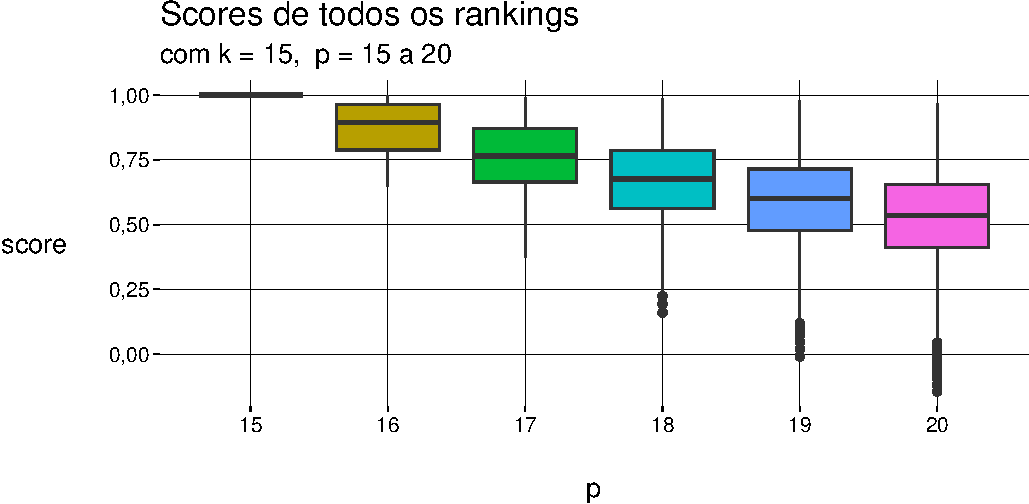
\includegraphics[width=1\textwidth,height=\textheight]{gerar-listas-e-rankings_files/figure-pdf/unnamed-chunk-10-1.pdf}
\end{center}

O argumento \texttt{reta}, opcional, especifica se deve ser incluída uma
reta de regressão linear via mínimos quadrados. O \emph{default} é
\texttt{TRUE}.

\begin{Shaded}
\begin{Highlighting}[]
\FunctionTok{plot}\NormalTok{(r, }\AttributeTok{reta =} \ConstantTok{FALSE}\NormalTok{)}
\end{Highlighting}
\end{Shaded}

\begin{center}
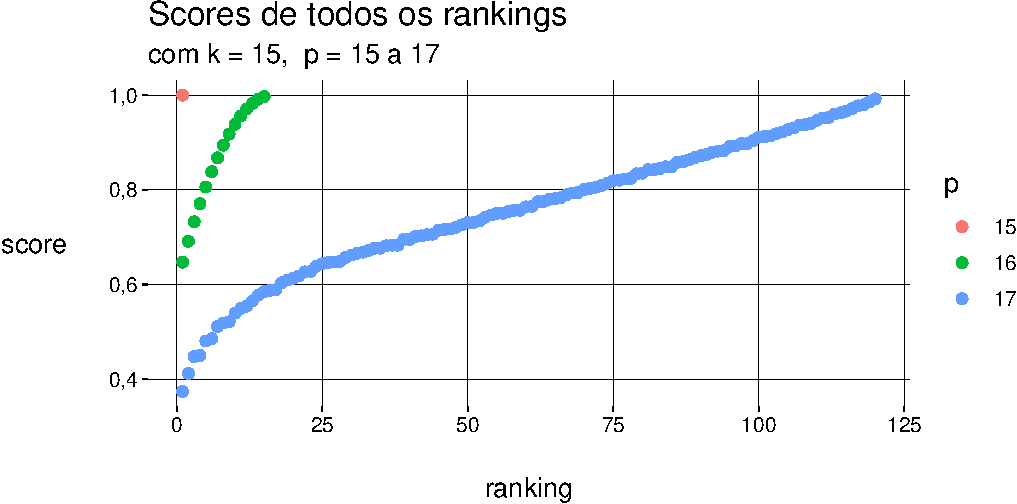
\includegraphics[width=1\textwidth,height=\textheight]{gerar-listas-e-rankings_files/figure-pdf/unnamed-chunk-11-1.pdf}
\end{center}

A função \texttt{plot} pode receber um argumento \texttt{fun}, opcional,
especificando uma função para calcular o \emph{score} deste
\emph{ranking} (i.e., alguma forma de correlação entre o \emph{ranking}
e a lista). O \emph{score} vai ser mostrado no título do gráfico.

A função passada em \texttt{fun} deve receber um objeto \texttt{rk} e
retornar o \emph{score} numérico.

\begin{Shaded}
\begin{Highlighting}[]
\FunctionTok{plot}\NormalTok{(}
\NormalTok{  r, }
  \AttributeTok{fun =}\NormalTok{ \textbackslash{}(r) \{ }
\NormalTok{    df }\OtherTok{\textless{}{-}} \FunctionTok{as\_tibble}\NormalTok{(r)}
    \FunctionTok{cor}\NormalTok{(df}\SpecialCharTok{$}\NormalTok{pos\_lista, df}\SpecialCharTok{$}\NormalTok{pos\_ranking) }\SpecialCharTok{\%\textgreater{}\%} \FunctionTok{round}\NormalTok{(}\DecValTok{2}\NormalTok{) }
\NormalTok{  \}}
\NormalTok{)}
\end{Highlighting}
\end{Shaded}

\begin{center}
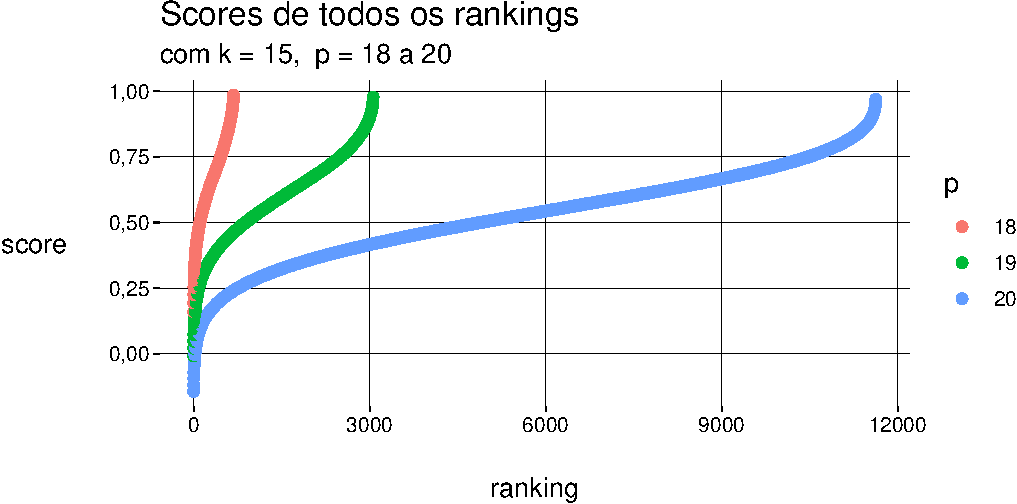
\includegraphics[width=1\textwidth,height=\textheight]{gerar-listas-e-rankings_files/figure-pdf/unnamed-chunk-12-1.pdf}
\end{center}

\subsection{\texorpdfstring{Criando uma \emph{tibble} com todos os
\emph{rankings}}{Criando uma tibble com todos os rankings}}\label{criando-uma-tibble-com-todos-os-rankings}

Dados valores de $p$ e $k$ (nesta ordem), a função
\texttt{criar\_df\_rankings()} retorna uma \emph{tibble} com todos os
$\binom{p - 1}{k - 1}$ \emph{rankings} possíveis, como objetos (S3) e
como \emph{strings}.

Todos os \emph{rankings} com $p = 8$ e $k = 5$:

\begin{Shaded}
\begin{Highlighting}[]
\FunctionTok{criar\_df\_rankings}\NormalTok{(}\DecValTok{8}\NormalTok{, }\DecValTok{5}\NormalTok{)}
\end{Highlighting}
\end{Shaded}

\begin{verbatim}
# A tibble: 35 x 4
   ranking ranking_str     k     p
   <list>  <chr>       <dbl> <dbl>
 1 <rk>    xxxx---x        5     8
 2 <rk>    xxx-x--x        5     8
 3 <rk>    xxx--x-x        5     8
 4 <rk>    xxx---xx        5     8
 5 <rk>    xx-xx--x        5     8
 6 <rk>    xx-x-x-x        5     8
 7 <rk>    xx-x--xx        5     8
 8 <rk>    xx--xx-x        5     8
 9 <rk>    xx--x-xx        5     8
10 <rk>    xx---xxx        5     8
11 <rk>    x-xxx--x        5     8
12 <rk>    x-xx-x-x        5     8
13 <rk>    x-xx--xx        5     8
14 <rk>    x-x-xx-x        5     8
15 <rk>    x-x-x-xx        5     8
16 <rk>    x-x--xxx        5     8
17 <rk>    x--xxx-x        5     8
18 <rk>    x--xx-xx        5     8
19 <rk>    x--x-xxx        5     8
20 <rk>    x---xxxx        5     8
21 <rk>    -xxxx--x        5     8
22 <rk>    -xxx-x-x        5     8
23 <rk>    -xxx--xx        5     8
24 <rk>    -xx-xx-x        5     8
25 <rk>    -xx-x-xx        5     8
26 <rk>    -xx--xxx        5     8
27 <rk>    -x-xxx-x        5     8
28 <rk>    -x-xx-xx        5     8
29 <rk>    -x-x-xxx        5     8
30 <rk>    -x--xxxx        5     8
31 <rk>    --xxxx-x        5     8
32 <rk>    --xxx-xx        5     8
33 <rk>    --xx-xxx        5     8
34 <rk>    --x-xxxx        5     8
35 <rk>    ---xxxxx        5     8
\end{verbatim}

Se for passado apenas o valor de $p$, a função retorna uma \emph{tibble}
com todos os \emph{rankings} possíveis de comprimento $p$ (com $k$
variando de $1$ até $p$). Exercício: quantos são?

Todos os \emph{rankings} com $p = 5$:

\begin{Shaded}
\begin{Highlighting}[]
\FunctionTok{criar\_df\_rankings}\NormalTok{(}\DecValTok{5}\NormalTok{)}
\end{Highlighting}
\end{Shaded}

\begin{verbatim}
# A tibble: 16 x 4
   ranking ranking_str     k     p
   <list>  <chr>       <int> <dbl>
 1 <rk>    ----x           1     5
 2 <rk>    x---x           2     5
 3 <rk>    -x--x           2     5
 4 <rk>    --x-x           2     5
 5 <rk>    ---xx           2     5
 6 <rk>    xx--x           3     5
 7 <rk>    x-x-x           3     5
 8 <rk>    x--xx           3     5
 9 <rk>    -xx-x           3     5
10 <rk>    -x-xx           3     5
11 <rk>    --xxx           3     5
12 <rk>    xxx-x           4     5
13 <rk>    xx-xx           4     5
14 <rk>    x-xxx           4     5
15 <rk>    -xxxx           4     5
16 <rk>    xxxxx           5     5
\end{verbatim}

Se você quiser a representação em \emph{string} usando unicode, basta
passar o argumento \texttt{unicode\ =\ TRUE}:

\begin{Shaded}
\begin{Highlighting}[]
\FunctionTok{criar\_df\_rankings}\NormalTok{(}\DecValTok{5}\NormalTok{, }\AttributeTok{unicode =} \ConstantTok{TRUE}\NormalTok{)}
\end{Highlighting}
\end{Shaded}

\begin{verbatim}
# A tibble: 16 x 4
   ranking ranking_str     k     p
   <list>  <chr>       <int> <dbl>
 1 <rk>    ••••✔           1     5
 2 <rk>    ✔•••✔           2     5
 3 <rk>    •✔••✔           2     5
 4 <rk>    ••✔•✔           2     5
 5 <rk>    •••✔✔           2     5
 6 <rk>    ✔✔••✔           3     5
 7 <rk>    ✔•✔•✔           3     5
 8 <rk>    ✔••✔✔           3     5
 9 <rk>    •✔✔•✔           3     5
10 <rk>    •✔•✔✔           3     5
11 <rk>    ••✔✔✔           3     5
12 <rk>    ✔✔✔•✔           4     5
13 <rk>    ✔✔•✔✔           4     5
14 <rk>    ✔•✔✔✔           4     5
15 <rk>    •✔✔✔✔           4     5
16 <rk>    ✔✔✔✔✔           5     5
\end{verbatim}

\bookmarksetup{startatroot}

\chapter{\texorpdfstring{O \emph{ranking} concorda com a lista?
Posições}{O ranking concorda com a lista? Posições}}\label{o-ranking-concorda-com-a-lista-posiuxe7uxf5es}

\section{\texorpdfstring{Usando $p$ como medida de
concordância}{Usando  como medida de concordância}}\label{usando-p}

Imagine que a lista de $k$ elementos foi definida por uma autoridade,
usando critérios que não conhecemos.

Em uma tentativa de descobrir esses critérios, construímos um modelo
para avaliar todos os elementos da população (que incluem os $k$
elementos da lista).

Nosso modelo produz um \emph{ranking} de todos os elementos. Para
facilitar, vamos supor que não há empates no \emph{ranking}.

Uma pergunta natural sobre a qualidade do \emph{ranking} produzido é

\begin{quote}
Quantas posições do \emph{ranking} são necessárias para incluir todos os
$k$ elementos da lista?
\end{quote}

A resposta é $p$, a posição, no \emph{ranking}, do elemento da lista com
pior classificação.

Aliás, é por isso que convencionamos, no capítulo anterior, que nossos
\emph{rankings} sempre terminam com um elemento da lista.

Um exemplo:

\begin{itemize}
\item
  A lista contém $k = 5$ elementos.
\item
  O \emph{ranking} $r_1$ é \texttt{xx-x-xx}, com $p = 7$.
\item
  O \emph{ranking} $r_2$ é \texttt{-xxxxx}, com $p = 6$.
\end{itemize}

Segundo a medida proposta aqui, $r_2$ é melhor que $r_1$.

Ou seja, quanto menor o valor de $p$, melhor o \emph{ranking}.

Embora comparar \emph{rankings} através de seus valores de $p$ seja
simples, podemos examinar medidas alternativas, que sejam mais finas que
esta.

Por exemplo, é discutível se os dois rankings \texttt{xx-\/-\/-x} e
\texttt{-\/-\/-xxx} devem ser considerados igualmente bons; no entanto,
ambos têm $p = 6$.

\section{\texorpdfstring{Usando $p$ e as posições dos elementos da
lista}{Usando  e as posições dos elementos da lista}}\label{usando-p-e-as-posiuxe7uxf5es-dos-elementos-da-lista}

\subsection{\texorpdfstring{Contando posições
\texttt{-}}{Contando posições -}}\label{contando-posiuxe7uxf5es--}

Dado um \emph{ranking} $r$ com $k$ e $p$, queremos definir uma função
$s(r)$ --- $s$ de \emph{score} --- com as seguintes características:

\begin{itemize}
\item
  Se $r$ não contiver ``\texttt{-}'', então $s(r) = 1$. Neste caso, $r$
  é um \emph{ranking} perfeito, que coincide com a lista (por exempĺo,
  \texttt{xxxxx}). Em casos assim, $k = p$. Vamos definir $s$ como sendo
  da forma

  \[
  s(r) = \frac k p + \cdots
  \]

  onde as reticências representam uma parcela que ainda vamos definir.
  Se $r$ for um \emph{ranking} perfeito, a parcela $k/p$ será $1$, e
  vamos definir a parcela restante para que seja igual a zero.
\item
  A parcela restante deve ter valor maior quanto melhor for o
  \emph{ranking}. Quanto mais próximos do fim do \emph{ranking}
  estiverem os caracteres ``\texttt{-}'', melhor ele será. Uma
  quantidade natural seria

  \[
  \frac{\operatorname{soma\_}}{\sum_{i = 1, p}i} 
  \quad=\quad 
  \frac{\operatorname{soma\_}}{p(p + 1) / 2}
  \quad=\quad 
  \frac{2\operatorname{soma\_}}{p(p + 1)}
  \]

  onde $\operatorname{soma\_}$ é a soma das posições ocupadas por
  ``\texttt{\_}'' em $r$.

  Como queríamos, quando $r$ for um \emph{ranking} perfeito,
  $\operatorname{soma\_} = 0$, e então $s(r) = 1$.
\item
  Mas também queremos que somente \emph{rankings} perfeitos tenham
  $s(r) = 1$. Para isso, considere que um \emph{ranking} mais próximo do
  perfeito é da forma

  \texttt{x...x-x}

  Ou seja, $k = p - 1$ e $\operatorname{soma\_} = p - 1$.

  Vamos multiplicar a segunda parcela por $\alpha$ de forma que
  $s(r) < 1$ para este \emph{ranking} quase perfeito:

  \[
  s(r) = \frac{p-1}{p} + \frac{2(p-1)}{p(p+1)} \cdot \alpha
  \]

  Então

  \[
  \begin{aligned}
    s(r) < 1 
    &\iff \frac{2(p-1)}{p(p+1)} \cdot \alpha < \frac1p \\
    &\iff 2 \alpha (p - 1) < p + 1 \\
    &\iff \alpha < \frac12 \cdot \frac{p + 1}{p - 1} \\
    &\iff \alpha = \frac1m \cdot \frac{p + 1}{p - 1} & (m > 2)
  \end{aligned}
  \]

  o que dá

  \[
  \begin{aligned}
  s(r) 
  &= \frac{k}{p} + \frac{2\operatorname{soma\_}}{p(p+1)} \cdot \alpha \\
  &= \frac{k}{p} + \frac{2\operatorname{soma\_}}{p(p+1)} \cdot 
    \frac1m \cdot \frac{p + 1}{p - 1} & (m > 2) \\
  &= \frac{k}{p} + \frac{2\operatorname{soma\_}}{p(p-1)} \cdot 
    \frac1m & (m > 2) \\
  &= \frac{k}{p} + \frac{\operatorname{soma\_}}{p(p-1)} \cdot 
    \frac2m & (m > 2)
  \end{aligned}
  \]

  Dependendo do valor de $m > 2$ escolhido, teremos medidas diferentes.

  A função que implementamos usa o \emph{default} de $m = 10$, mas
  valores diferentes podem ser passados.
\end{itemize}

\begin{Shaded}
\begin{Highlighting}[]
\NormalTok{r }\OtherTok{\textless{}{-}} \FunctionTok{rk}\NormalTok{(}\StringTok{\textquotesingle{}xxx{-}x\textquotesingle{}}\NormalTok{)}
\FunctionTok{s}\NormalTok{(r)}
\end{Highlighting}
\end{Shaded}

\begin{verbatim}
[1] 0,84
\end{verbatim}

Para $p = 8$, alguns exemplos:

\begin{Shaded}
\begin{Highlighting}[]
\FunctionTok{s}\NormalTok{(}
  \FunctionTok{list}\NormalTok{(}
    \FunctionTok{rk}\NormalTok{(}\StringTok{\textquotesingle{}xxxxxxxx\textquotesingle{}}\NormalTok{),}
    \FunctionTok{rk}\NormalTok{(}\StringTok{\textquotesingle{}xxxxxx{-}x\textquotesingle{}}\NormalTok{),}
    \FunctionTok{rk}\NormalTok{(}\StringTok{\textquotesingle{}{-}xxxxxxx\textquotesingle{}}\NormalTok{)}
\NormalTok{  )}
\NormalTok{)}
\end{Highlighting}
\end{Shaded}

\begin{verbatim}
[1] 1,0000000 0,9000000 0,8785714
\end{verbatim}

Eis todos os \emph{rankings} de comprimento $8$, com suas pontuações:

\begin{longtable*}{lr}
\toprule
ranking\_str & s \\ 
\midrule\addlinespace[2.5pt]
xxxxxxxx & 1,0000000 \\ 
xxxxxx-x & 0,9000000 \\ 
xxxxx-xx & 0,8964286 \\ 
xxxx-xxx & 0,8928571 \\ 
xxx-xxxx & 0,8892857 \\ 
xx-xxxxx & 0,8857143 \\ 
x-xxxxxx & 0,8821429 \\ 
-xxxxxxx & 0,8785714 \\ 
xxxxx--x & 0,7964286 \\ 
xxxx-x-x & 0,7928571 \\ 
xxxx--xx & 0,7892857 \\ 
xxx-xx-x & 0,7892857 \\ 
xxx-x-xx & 0,7857143 \\ 
xx-xxx-x & 0,7857143 \\ 
xxx--xxx & 0,7821429 \\ 
xx-xx-xx & 0,7821429 \\ 
x-xxxx-x & 0,7821429 \\ 
xx-x-xxx & 0,7785714 \\ 
x-xxx-xx & 0,7785714 \\ 
-xxxxx-x & 0,7785714 \\ 
xx--xxxx & 0,7750000 \\ 
x-xx-xxx & 0,7750000 \\ 
-xxxx-xx & 0,7750000 \\ 
x-x-xxxx & 0,7714286 \\ 
-xxx-xxx & 0,7714286 \\ 
x--xxxxx & 0,7678571 \\ 
-xx-xxxx & 0,7678571 \\ 
-x-xxxxx & 0,7642857 \\ 
--xxxxxx & 0,7607143 \\ 
xxxx---x & 0,6892857 \\ 
xxx-x--x & 0,6857143 \\ 
xxx--x-x & 0,6821429 \\ 
xx-xx--x & 0,6821429 \\ 
xxx---xx & 0,6785714 \\ 
xx-x-x-x & 0,6785714 \\ 
x-xxx--x & 0,6785714 \\ 
xx-x--xx & 0,6750000 \\ 
xx--xx-x & 0,6750000 \\ 
x-xx-x-x & 0,6750000 \\ 
-xxxx--x & 0,6750000 \\ 
xx--x-xx & 0,6714286 \\ 
x-xx--xx & 0,6714286 \\ 
x-x-xx-x & 0,6714286 \\ 
-xxx-x-x & 0,6714286 \\ 
xx---xxx & 0,6678571 \\ 
x-x-x-xx & 0,6678571 \\ 
x--xxx-x & 0,6678571 \\ 
-xxx--xx & 0,6678571 \\ 
-xx-xx-x & 0,6678571 \\ 
x-x--xxx & 0,6642857 \\ 
x--xx-xx & 0,6642857 \\ 
-xx-x-xx & 0,6642857 \\ 
-x-xxx-x & 0,6642857 \\ 
x--x-xxx & 0,6607143 \\ 
-xx--xxx & 0,6607143 \\ 
-x-xx-xx & 0,6607143 \\ 
--xxxx-x & 0,6607143 \\ 
x---xxxx & 0,6571429 \\ 
-x-x-xxx & 0,6571429 \\ 
--xxx-xx & 0,6571429 \\ 
-x--xxxx & 0,6535714 \\ 
--xx-xxx & 0,6535714 \\ 
--x-xxxx & 0,6500000 \\ 
---xxxxx & 0,6464286 \\ 
xxx----x & 0,5785714 \\ 
xx-x---x & 0,5750000 \\ 
xx--x--x & 0,5714286 \\ 
x-xx---x & 0,5714286 \\ 
xx---x-x & 0,5678571 \\ 
x-x-x--x & 0,5678571 \\ 
-xxx---x & 0,5678571 \\ 
xx----xx & 0,5642857 \\ 
x-x--x-x & 0,5642857 \\ 
x--xx--x & 0,5642857 \\ 
-xx-x--x & 0,5642857 \\ 
x-x---xx & 0,5607143 \\ 
x--x-x-x & 0,5607143 \\ 
-xx--x-x & 0,5607143 \\ 
-x-xx--x & 0,5607143 \\ 
x--x--xx & 0,5571429 \\ 
x---xx-x & 0,5571429 \\ 
-xx---xx & 0,5571429 \\ 
-x-x-x-x & 0,5571429 \\ 
--xxx--x & 0,5571429 \\ 
x---x-xx & 0,5535714 \\ 
-x-x--xx & 0,5535714 \\ 
-x--xx-x & 0,5535714 \\ 
--xx-x-x & 0,5535714 \\ 
x----xxx & 0,5500000 \\ 
-x--x-xx & 0,5500000 \\ 
--xx--xx & 0,5500000 \\ 
--x-xx-x & 0,5500000 \\ 
-x---xxx & 0,5464286 \\ 
--x-x-xx & 0,5464286 \\ 
---xxx-x & 0,5464286 \\ 
--x--xxx & 0,5428571 \\ 
---xx-xx & 0,5428571 \\ 
---x-xxx & 0,5392857 \\ 
----xxxx & 0,5357143 \\ 
xx-----x & 0,4642857 \\ 
x-x----x & 0,4607143 \\ 
x--x---x & 0,4571429 \\ 
-xx----x & 0,4571429 \\ 
x---x--x & 0,4535714 \\ 
-x-x---x & 0,4535714 \\ 
x----x-x & 0,4500000 \\ 
-x--x--x & 0,4500000 \\ 
--xx---x & 0,4500000 \\ 
x-----xx & 0,4464286 \\ 
-x---x-x & 0,4464286 \\ 
--x-x--x & 0,4464286 \\ 
-x----xx & 0,4428571 \\ 
--x--x-x & 0,4428571 \\ 
---xx--x & 0,4428571 \\ 
--x---xx & 0,4392857 \\ 
---x-x-x & 0,4392857 \\ 
---x--xx & 0,4357143 \\ 
----xx-x & 0,4357143 \\ 
----x-xx & 0,4321429 \\ 
-----xxx & 0,4285714 \\ 
x------x & 0,3464286 \\ 
-x-----x & 0,3428571 \\ 
--x----x & 0,3392857 \\ 
---x---x & 0,3357143 \\ 
----x--x & 0,3321429 \\ 
-----x-x & 0,3285714 \\ 
------xx & 0,3250000 \\ 
-------x & 0,2250000 \\ 
\bottomrule
\end{longtable*}

Perceba que pode haver empates: \texttt{xxxx-\/-xx} e \texttt{xxx-xx-x}
têm o mesmo valor de $s$. É razoável achar que estes dois
\emph{rankings} têm a mesma qualidade.

\subsection{\texorpdfstring{Comparando \emph{rankings} com valores
diferentes de
$p$}{Comparando rankings com valores diferentes de }}\label{comparando-rankings-com-valores-diferentes-de-p}

Como a lista é dada e fixa, só faz sentido, na prática, comparar
\emph{rankings} com o mesmo valor de $k$.

Vamos examinar, para uma lista com $k = 2$, os \emph{rankings} possíveis
com $p$ variando de $2$ a $10$.

São $45$ \emph{rankings}:

\begin{longtable*}{lrr}
\toprule
ranking\_str & p & s \\ 
\midrule\addlinespace[2.5pt]
xx & 2 & 1,0000000 \\ 
x-x & 3 & 0,7333333 \\ 
-xx & 3 & 0,7000000 \\ 
x--x & 4 & 0,5833333 \\ 
-x-x & 4 & 0,5666667 \\ 
--xx & 4 & 0,5500000 \\ 
x---x & 5 & 0,4900000 \\ 
-x--x & 5 & 0,4800000 \\ 
--x-x & 5 & 0,4700000 \\ 
---xx & 5 & 0,4600000 \\ 
x----x & 6 & 0,4266667 \\ 
-x---x & 6 & 0,4200000 \\ 
--x--x & 6 & 0,4133333 \\ 
---x-x & 6 & 0,4066667 \\ 
----xx & 6 & 0,4000000 \\ 
x-----x & 7 & 0,3809524 \\ 
-x----x & 7 & 0,3761905 \\ 
--x---x & 7 & 0,3714286 \\ 
---x--x & 7 & 0,3666667 \\ 
----x-x & 7 & 0,3619048 \\ 
-----xx & 7 & 0,3571429 \\ 
x------x & 8 & 0,3464286 \\ 
-x-----x & 8 & 0,3428571 \\ 
--x----x & 8 & 0,3392857 \\ 
---x---x & 8 & 0,3357143 \\ 
----x--x & 8 & 0,3321429 \\ 
-----x-x & 8 & 0,3285714 \\ 
------xx & 8 & 0,3250000 \\ 
x-------x & 9 & 0,3194444 \\ 
-x------x & 9 & 0,3166667 \\ 
--x-----x & 9 & 0,3138889 \\ 
---x----x & 9 & 0,3111111 \\ 
----x---x & 9 & 0,3083333 \\ 
-----x--x & 9 & 0,3055556 \\ 
------x-x & 9 & 0,3027778 \\ 
-------xx & 9 & 0,3000000 \\ 
x--------x & 10 & 0,2977778 \\ 
-x-------x & 10 & 0,2955556 \\ 
--x------x & 10 & 0,2933333 \\ 
---x-----x & 10 & 0,2911111 \\ 
----x----x & 10 & 0,2888889 \\ 
-----x---x & 10 & 0,2866667 \\ 
------x--x & 10 & 0,2844444 \\ 
-------x-x & 10 & 0,2822222 \\ 
--------xx & 10 & 0,2800000 \\ 
\bottomrule
\end{longtable*}

Os gráficos abaixo mostram os \emph{scores} atribuídos para todos os
\emph{rankings} com $k = 2$ e $p$ variando de $2$ a $10$, separados por
valores de $p$:

\begin{center}
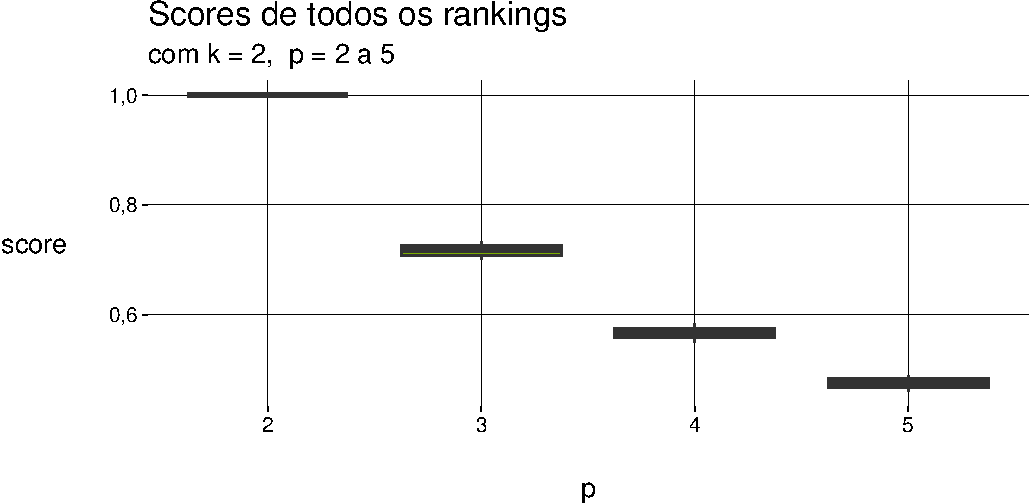
\includegraphics[width=1\textwidth,height=\textheight]{usando-posicoes_files/figure-pdf/unnamed-chunk-7-1.pdf}
\end{center}

\begin{center}
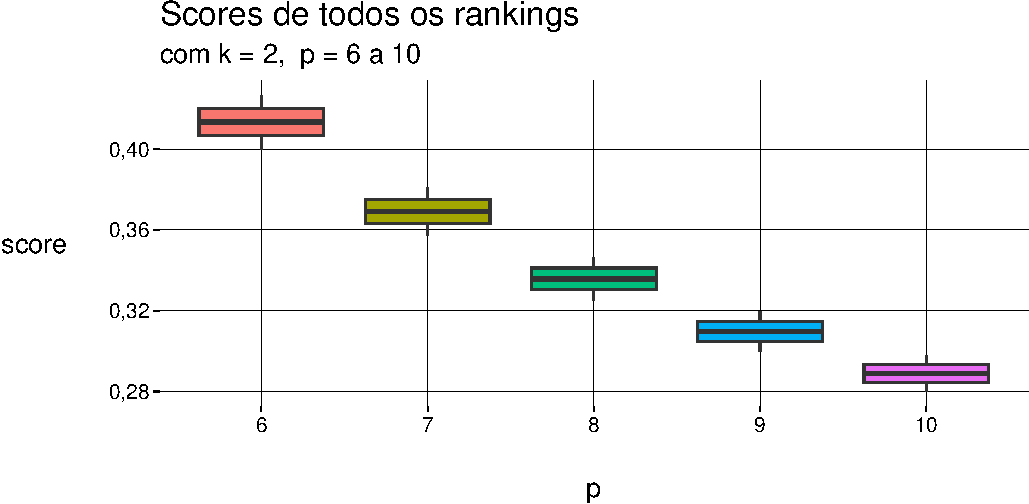
\includegraphics[width=1\textwidth,height=\textheight]{usando-posicoes_files/figure-pdf/unnamed-chunk-8-1.pdf}
\end{center}

\begin{center}
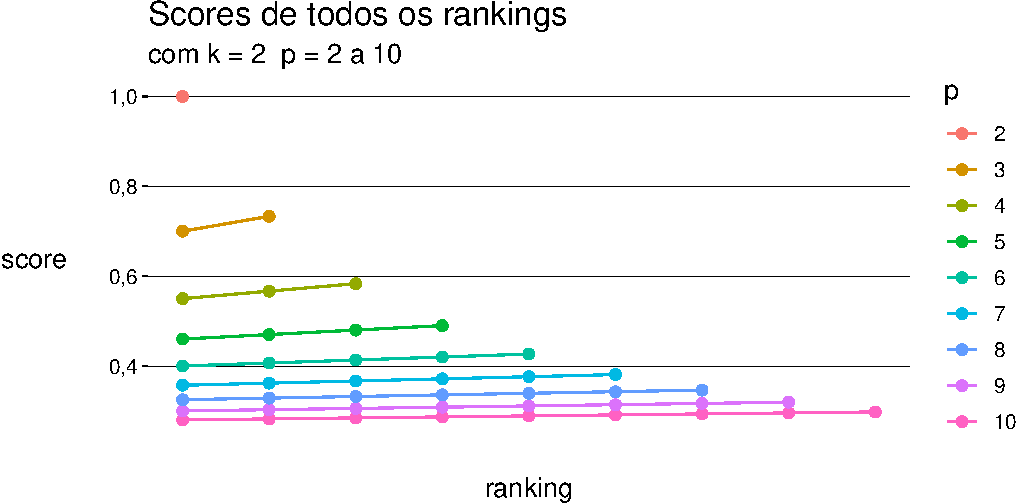
\includegraphics[width=1\textwidth,height=\textheight]{usando-posicoes_files/figure-pdf/unnamed-chunk-9-1.pdf}
\end{center}

\subsection{\texorpdfstring{Outros valores de
$m$}{Outros valores de }}\label{outros-valores-de-m}

O valor de $m$ altera a função $s()$ de maneira a permitir
sobreposições:

Para $m = 5$:

Vamos examinar, para uma lista com $k = 2$, os \emph{rankings} possíveis
com $p$ variando de $2$ a $10$.

São $45$ \emph{rankings}:

\begin{longtable*}{lrr}
\toprule
ranking\_str & p & s \\ 
\midrule\addlinespace[2.5pt]
xx & 2 & 1,0000000 \\ 
x-x & 3 & 0,8000000 \\ 
-xx & 3 & 0,7333333 \\ 
x--x & 4 & 0,6666667 \\ 
-x-x & 4 & 0,6333333 \\ 
--xx & 4 & 0,6000000 \\ 
x---x & 5 & 0,5800000 \\ 
-x--x & 5 & 0,5600000 \\ 
--x-x & 5 & 0,5400000 \\ 
---xx & 5 & 0,5200000 \\ 
x----x & 6 & 0,5200000 \\ 
-x---x & 6 & 0,5066667 \\ 
--x--x & 6 & 0,4933333 \\ 
---x-x & 6 & 0,4800000 \\ 
x-----x & 7 & 0,4761905 \\ 
----xx & 6 & 0,4666667 \\ 
-x----x & 7 & 0,4666667 \\ 
--x---x & 7 & 0,4571429 \\ 
---x--x & 7 & 0,4476190 \\ 
x------x & 8 & 0,4428571 \\ 
----x-x & 7 & 0,4380952 \\ 
-x-----x & 8 & 0,4357143 \\ 
--x----x & 8 & 0,4285714 \\ 
-----xx & 7 & 0,4285714 \\ 
---x---x & 8 & 0,4214286 \\ 
x-------x & 9 & 0,4166667 \\ 
----x--x & 8 & 0,4142857 \\ 
-x------x & 9 & 0,4111111 \\ 
-----x-x & 8 & 0,4071429 \\ 
--x-----x & 9 & 0,4055556 \\ 
------xx & 8 & 0,4000000 \\ 
---x----x & 9 & 0,4000000 \\ 
x--------x & 10 & 0,3955556 \\ 
----x---x & 9 & 0,3944444 \\ 
-x-------x & 10 & 0,3911111 \\ 
-----x--x & 9 & 0,3888889 \\ 
--x------x & 10 & 0,3866667 \\ 
------x-x & 9 & 0,3833333 \\ 
---x-----x & 10 & 0,3822222 \\ 
-------xx & 9 & 0,3777778 \\ 
----x----x & 10 & 0,3777778 \\ 
-----x---x & 10 & 0,3733333 \\ 
------x--x & 10 & 0,3688889 \\ 
-------x-x & 10 & 0,3644444 \\ 
--------xx & 10 & 0,3600000 \\ 
\bottomrule
\end{longtable*}

\begin{center}
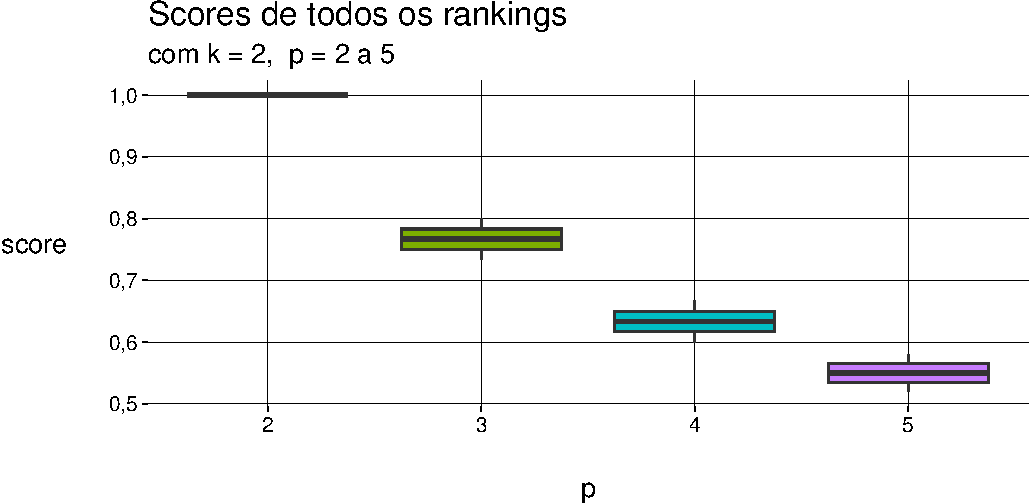
\includegraphics[width=1\textwidth,height=\textheight]{usando-posicoes_files/figure-pdf/unnamed-chunk-12-1.pdf}
\end{center}

\begin{center}
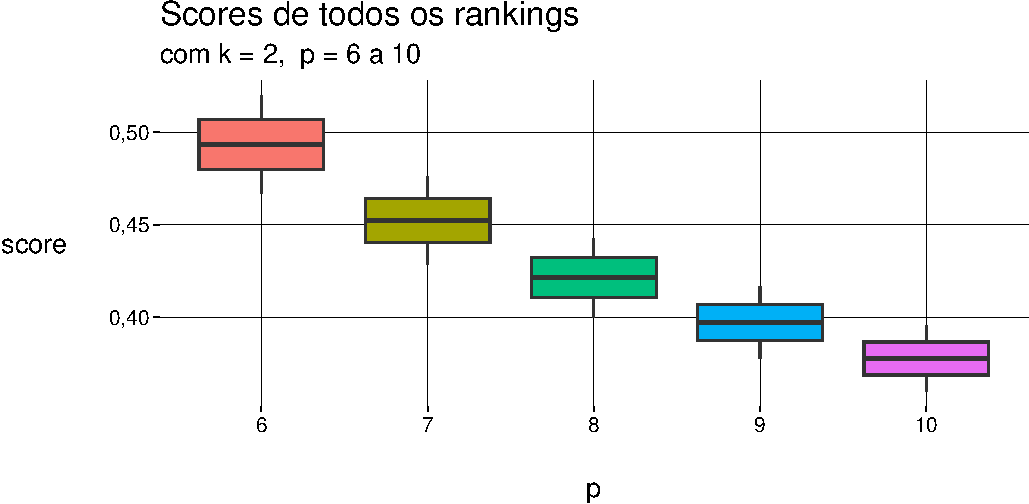
\includegraphics[width=1\textwidth,height=\textheight]{usando-posicoes_files/figure-pdf/unnamed-chunk-13-1.pdf}
\end{center}

\begin{center}
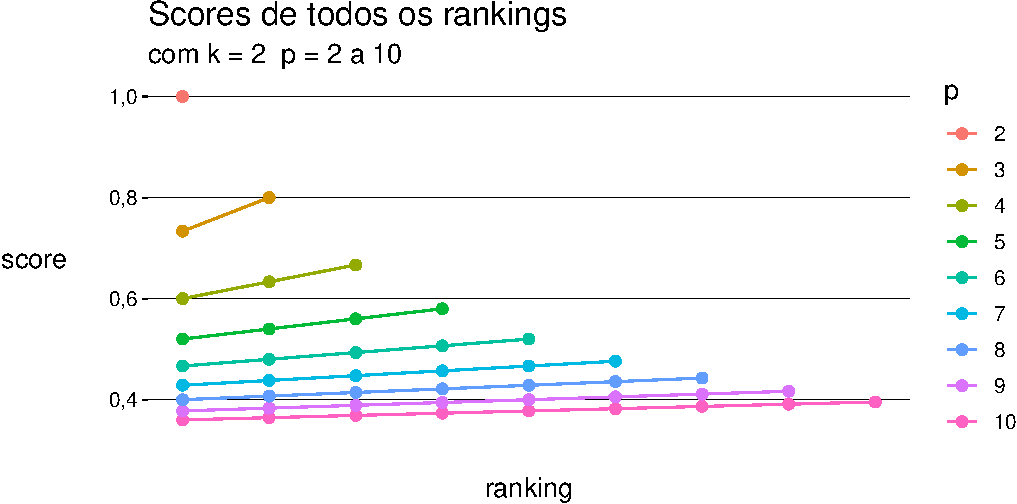
\includegraphics[width=1\textwidth,height=\textheight]{usando-posicoes_files/figure-pdf/unnamed-chunk-14-1.pdf}
\end{center}

\bookmarksetup{startatroot}

\chapter{Precisão e revocação}\label{precisuxe3o-e-revocauxe7uxe3o}

\section{Contexto}\label{contexto}

Precisão e revocação são métricas usadas em problemas de classificação.

No nosso contexto, vamos considerar os $k$ elementos da lista como sendo
aqueles cuja classe é a \emph{positiva}, i.e., a lista nos dá a verdade
fundamental (\emph{ground truth}); todos os outros elementos do universo
têm classe \emph{negativa}.

Em vez de produzir um \emph{ranking}, nosso modelo vai produzir uma
\emph{classificação binária}, rotulando alguns elementos como positivos
e alguns elementos como negativos.

\section{Definições}\label{definiuxe7uxf5es}

Precisão e revocação são noções ligadas a reconhecimento de padrões e
recuperação de informações.

Vamos usar uma tabela de contingência binária como na
Figura~\ref{fig-tab-cont}, retirada de Powers (2007).

\begin{figure}[htb]

\centering{

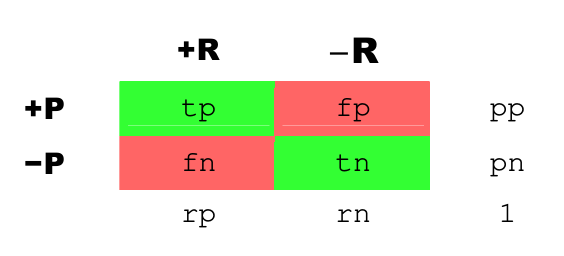
\includegraphics[width=0.6\textwidth,height=\textheight]{images/contingency-table.png}

}

\caption{\label{fig-tab-cont}Tabela de contingência binária}

\end{figure}%

Aqui, as colunas \textbf{+R} e \textbf{-R} representam a verdade
fundamental (positivos e negativos). As linhas \textbf{+P} e \textbf{-P}
representam as classes previstas pelo modelo. Além disso,

\begin{itemize}
\tightlist
\item
  \texttt{tp} = \emph{true positives}
\item
  \texttt{fp} = \emph{false positives}
\item
  \texttt{fn} = \emph{false negatives}
\item
  \texttt{tn} = \emph{true negatives}
\item
  \texttt{rp} = \emph{real positives}
\item
  \texttt{rn} = \emph{real negatives}
\item
  \texttt{pp} = \emph{predicted positive}
\item
  \texttt{pn} = \emph{predicted negative}
\end{itemize}

As células verdes correspondem a previsões corretas, as vermelhas a
previsões erradas.

\begin{tcolorbox}[enhanced jigsaw, toprule=.15mm, bottomrule=.15mm, coltitle=black, left=2mm, colframe=quarto-callout-note-color-frame, titlerule=0mm, leftrule=.75mm, bottomtitle=1mm, title=\textcolor{quarto-callout-note-color}{\faInfo}\hspace{0.5em}{Recall}, breakable, rightrule=.15mm, colbacktitle=quarto-callout-note-color!10!white, toptitle=1mm, arc=.35mm, opacitybacktitle=0.6, opacityback=0, colback=white]

\emph{Recall} (ou \emph{sensibilidade}, ou \emph{revocação}) é a
proporção de positivos verdadeiros que são previstos como positivos. Em
ROC, é a taxa de positivos verdadeiros (\emph{true positive rate},
\texttt{tpr}):

\[
\text{recall} = \texttt{tpr} = \frac{\texttt{tp}}{\texttt{rp}}
\]

\emph{Recall} só usa informação da coluna \textbf{+R}.

\end{tcolorbox}

\begin{tcolorbox}[enhanced jigsaw, toprule=.15mm, bottomrule=.15mm, coltitle=black, left=2mm, colframe=quarto-callout-note-color-frame, titlerule=0mm, leftrule=.75mm, bottomtitle=1mm, title=\textcolor{quarto-callout-note-color}{\faInfo}\hspace{0.5em}{Precisão}, breakable, rightrule=.15mm, colbacktitle=quarto-callout-note-color!10!white, toptitle=1mm, arc=.35mm, opacitybacktitle=0.6, opacityback=0, colback=white]

\emph{Precisão} (ou \emph{confiança}) é a proporção de elementos
previstos como positivos que são realmente positivos. Pode ser chamada
de \emph{true positive accuracy} (\texttt{tpa}):

\[
\text{precisão} = \texttt{tpa} = \frac{\texttt{tp}}{\texttt{pp}}
\]

Em ROC, que não usa métricas envolvendo quantidades de colunas
diferentes da tabela de contingência --- ver Fawcett (2006) --- precisão
não é usada.

\emph{Precisão} só usa informação da linha \textbf{+P}.

\end{tcolorbox}

Várias questões sobre estas duas métricas são abordadas em Powers
(2007), incluindo os seus vieses. Vamos ignorar estas questões por
enquanto.

\section{\texorpdfstring{Exemplo sem
\emph{threshold}}{Exemplo sem threshold}}\label{exemplo-sem-threshold}

Considere o \emph{ranking} \texttt{xx-\/-\/-x-xx}, com $p = 9$ e
$k = 5$.

Até agora, nossos \emph{rankings} não vêm acompanhados de um valor
limite (\emph{threshold}) acima do qual os elementos são previstos como
positivos e abaixo do qual os elementos são previstos como negativos.

Vamos considerar que todos os $p$ elementos representados no
\emph{string} são previstos como positivos. Isto significa que não há
falsos negativos.

Até agora, nossa representação para \emph{rankings} não leva em conta o
total de elementos da população. Vamos chamar este total de $n$.

\begin{itemize}
\item
  Os elementos que não aparecem neste \emph{string} são em número de
  $n - p = n - 9$.
\item
  Os \emph{real positives} são em número de $\texttt{rp} = k = 5$.
\item
  Os \emph{real negatives} são em número de
  $\texttt{rn} = n - k = n - 5$.
\item
  Os \emph{true positives} são em número de $\texttt{tp} = k = 5$.
\item
  Os \emph{predicted positive} são em número de $\texttt{pp} = p = 9$.
\item
  Os \emph{false negatives} são $\texttt{fn} = 0$.
\item
  Os \emph{false positives} são em número de
  $\texttt{fp} = p - k = 9 - 5 = 4$.
\end{itemize}

A tabela fica:

\begin{longtable*}{lrll}
\toprule
  & +R & -R & Total \\ 
\midrule\addlinespace[2.5pt]
+P & 5 & 4 & 9 \\ 
-P & 0 & n - p & n - p \\ 
Total & 5 & n - k & n \\ 
\bottomrule
\end{longtable*}

Daí, o \emph{recall} sempre vai ser $1$, e a precisão é simplesmente

\[
\frac kp = \frac59
\]

Mas, uma vez fixado o valor de $k$, isto equivale a atribuir o mesmo
\emph{score} a todos os \emph{rankings} com o mesmo valor de $p$. Não é
interessante.

\bookmarksetup{startatroot}

\chapter*{Referências}\label{referuxeancias}
\addcontentsline{toc}{chapter}{Referências}

\markboth{Referências}{Referências}

\phantomsection\label{refs}
\begin{CSLReferences}{1}{0}
\bibitem[\citeproctext]{ref-fawcett06:_roc}
Fawcett, Tom. 2006. "An introduction to ROC analysis". \emph{Pattern
Recognition Letters} 27, no.8: 861--74.
\url{https://doi.org/10.1016/j.patrec.2005.10.010}.

\bibitem[\citeproctext]{ref-powers07:precision_recall}
Powers, David M. W. 2007. "Evaluation: From Precision, Recall and
F-Factor to ROC, Informedness, Markedness \& Correlation". SIE-07-001.
School of Informatics; Engineering; Flinders University.
\url{http://david.wardpowers.info/BM/index.htm}.

\end{CSLReferences}



\end{document}
